\documentclass{cumcmthesis}
% \documentclass[withoutpreface,bwprint]{cumcmthesis} %去掉封面与编号页，电子版提交的时候使用。


\usepackage[framemethod=TikZ]{mdframed}
\usepackage{url}   % 网页链接
\usepackage{subcaption} % 子标题
\usepackage{comment}
\title{客机水面迫降时的姿态}
\tihao{A}
\baominghao{432112344321}
\schoolname{西安电子科技大学}
\membera{ 王潇晗 }
\memberb{ 刘懿萱 }
\memberc{ 王碧凡 }
\supervisor{ 宋月 }%辅导老师
\yearinput{2025}
\monthinput{8}
\dayinput{18}

\begin{document}

 \maketitle
 \begin{abstract}%摘要在这里写

\keywords{\TeX{}\quad  图片\quad   表格\quad  公式}
\end{abstract}

%目录  2019 明确不要目录，我觉得这个规定太好了
%\tableofcontents

%\newpage

\section{问题重述}
\subsection{问题背景}
在航空运营中, 客机因突发故障, 如发动机失效、飞鸟撞击等, 导致失去动力而被迫进行水面迫降的情况虽较为罕见, 但具有极高的危险性. 此类事故中, 客机与水面的接触姿态、航向等因素直接影响机身结构完整性、乘客生存概率及救援效率. 

2009年1月15日, 美国全美航空公司 (US Airways)第1549航班 (空中客车A320客机)从纽约长岛拉瓜迪亚机场起飞约90秒后遭飞鸟撞击, 导致两个发动机损坏. 机长凭借出色的驾驶技术和冷静判断, 将飞机成功迫降在纽约哈德逊河河面, 机上155人在飞机沉没前全部获救, 仅78人受伤, 无人死亡. 该案例充分体现了合理迫降策略对事故结果的关键影响. 

对于越洋飞行航班, 在海面迫降的情况更为复杂. 海面环境受风浪影响显著, 波浪的高度、周期、方向等因素会进一步增加迫降难度, 对客机的姿态控制、航向选择提出更高要求. 因此, 针对不同水面环境（平静水面与有风浪海面）建立科学的数学模型, 分析最优迫降策略具有重要的理论与实践意义. 

\subsection{问题提出}
基于上述背景，需结合实际情况建立数学模型，分析以下问题：

1. 第一阶段问题：大型客机因失去动力在平静水面进行迫降时，具有相当大的危险性。需建立合理的数学模型，对客机在平静水面上的迫降进行分析，指出客机在河面上迫降时，以何种姿态接触水面是相对最好的选择。

2. 第二阶段问题：在越洋飞行中，个别航班曾因重大故障或意外原因被迫在海面迫降。有风浪条件下，飞机在海面的迫降难度和危险性更大。需建立合理的数学模型，对客机在海面的迫降进行分析，指出在有风浪的条件下，飞机以何种姿态和航向接触海面是相对安全的选择。
\section{问题分析}

客机水面迫降是航空安全领域中极具挑战性的复杂问题，其核心在于通过优化飞机接触水面时的姿态与航向，最大限度降低机身结构损伤风险并保障乘客安全。本研究需针对平静水面与有风浪海面海面两种两种典型场景，系统分析影响迫降安全性的关键因素及作用机制。

\subsection{问题一: 平静水面迫降问题分析}

平静水面环境下, 迫降安全性主要取决于飞机接触水面瞬间的姿态参数与运动状态决定. 此时水面可近似为刚性平面, 冲击力的分布与大小直接由机身接触方式决定. 分析表明, 该场景下的核心矛盾在于: 

- 姿态与冲击力的平衡: 机头过度抬起 (大俯仰角)会导致机尾率先接触水面, 虽可避免机头直接撞击, 但可能因尾部结构过载引发断裂: 而俯仰角过小或负角度 (机头俯冲) 则会使机头先入水, 巨大的冲击力易造成驾驶舱损毁及前部结构解体.

- 速度与缓冲的权衡: 水平速度过高会增加滑行阶段的摩擦阻力与姿态失稳风险，垂直速度过大会加剧冲击过载，但过低的水平速度可能导致飞机失速，丧失姿态控制能力。

- 结构强度与乘客耐受的匹配: 机身材料的弯曲强度极限 (以最大弯矩表征) 与乘客的加速度耐受阈值 (竖直方向约3g, 水平方向约5g) 构成双重约束, 需通过姿态优化使两者同时处于安全范围.

研究需重点建立俯仰角与侧倾角 (理想状态为0°) 对冲击力、弯矩及加速度的定量影响模型, 通过多目标优化确定最佳最佳姿态参数. 

\subsection{问题二: 有风浪海面迫降问题分析}

有风浪条件下, 海面的动态特性使迫降问题复杂度显著提升, 需在平静水面模型基础上引入波浪-机身相互作用机制. 关键问题包括:

- 波浪参数的影响: 波浪高度 ($H_w$) 决定了机身接触水面时的瞬时高差, 周期 ($T_w$) 影响接触时机的选择, 波长 ($\lambda$) 则与机身长度耦合, 决定是否可能同时接触波峰与波谷. 

- 相对速度的修正: 波浪运动导致水质点产生周期性水平与垂直速度 ($u_w, w_w$), 使飞机与水面的相对速度 ($v_h', v_v', v_s'$) 不同于绝对速度, 显著改变冲击力大小与方向. 

- 航向角的选择: 机身纵轴与波浪传播方向的夹角 ($\phi$) 直接影响侧向力与侧倾力矩 ($M_s$). 顺浪 ($\phi \approx 0^\circ$) 可减小水平相对速度, 逆浪会增大冲击载荷, 横浪则易引发侧翻.

- 动态接触的不确定性: 波浪的周期性起伏使机身接触水面的位置与面积随时间动态变化, 导致冲击力分布不稳定, 增加结构局部过载风险.

该场景需构建考虑波浪运动学特性的扩展模型, 分析俯仰角、侧倾角与航向角的协同优化策略, 在动态环境中实现安全系数最大化.

\subsection{问题关联与核心差异}

两类问题的本质均为多约束条件下的姿态优化问题, 但存在显著差异: 平静水面问题可简化为刚体与刚性平面的冲击动力学问题, 核心是静态姿态参数优化; 而风浪海面问题需考虑弹性体与刚体的动态耦合作用, 引入航向角作为关键变量, 优化目标更复杂, 约束条件更严苛. 研究需在统一的安全评估框架下, 分别建立针对性模型, 揭示不同环境下的最优迫降机理. 
    
\section{模型假设与符号说明}
\subsection{模型假设}
1. 假设客机在迫降过程中可简化为刚体, 忽略机身局部形变对整体姿态的影响. 

2. 平静水面条件下, 将水面视为理想刚性平面, 不考虑水流扰动对冲击力的影响. 

3. 风浪条件下, 波浪运动符合线性波浪模型, 水质点做周期性圆周运动, 且水深满足深水条件 (\( h \gg \lambda \)). 

4. 迫降过程中侧倾角控制为0 (机翼水平), 仅考虑俯仰角和航向角对安全性的影响. 

5. 机身材料均匀, 结构强度以屈服强度为临界指标, 忽略疲劳损伤累积效应. 

6. 乘客过载耐受极限为: 竖直方向不超过3g, 水平方向不超过5g, 侧向不超过6g (\( g \)为重力加速度). 

\subsection{符号说明}
\begin{table}[H]
\centering
\caption{主要符号及物理意义}
\label{tab:symbol}
\begin{tabular}{|c|c|c|}
\hline
\textbf{符号类别} & \textbf{符号} & \textbf{物理意义及单位} \\
\hline
\multirow{6}{*}{\textbf{基本参数}} 
& \( m \) & 客机总质量 (\( \text{kg} \)) \\ \cline{2-3}
& \( L \) & 机身长度 (\( \text{m} \)) \\ \cline{2-3}
& \( W \) & 机身宽度 (\( \text{m} \)) \\ \cline{2-3}
& \( B \) & 机翼展长 (\( \text{m} \)) \\ \cline{2-3}
& \( S \) & 机翼面积(\( \text{m}^2 \)) \\ \cline{2-3}
& \( g \) & 重力加速度(\( 9.81\ \text{m/s}^2 \))\\
\hline
\multirow{5}{*}{\textbf{材料参数}} 
& \( \sigma_s \) & 机身材料屈服强度 (\( \text{Pa} \)) \\ \cline{2-3}
& \( E \) & 机身材料弹性模量 (\( \text{Pa} \)) \\ \cline{2-3}
& \( D \) & 机身截面外径 (\( \text{m} \)) \\ \cline{2-3}
& \( d \) & 机身截面内径 (\( \text{m} \)) \\ \cline{2-3}
& \( t \) & 机身壁厚 (\( t=(D-d)/2 \), m) \\
\hline
\multirow{3}{*}{\textbf{姿态参数}} 
& \( \theta \) & 俯仰角（机身纵轴与水面夹角，°） \\ \cline{2-3}
& \( \alpha \) & 侧倾角（机翼平面与水面夹角，°） \\ \cline{2-3}
& \( \phi \) & 航向角（机身与波浪方向夹角，°） \\
\hline
\end{tabular}
\end{table}

\begin{table}[H]
\centering
\caption{主要符号及物理意义}
\label{tab:symbol}
\begin{tabular}{|c|c|c|}
\hline
\multirow{6}{*}{\textbf{速度参数}} 
& \( v \) & 飞机合速度 (\( \text{m/s} \)) \\ \cline{2-3}
& \( v_h \) & 水平速度 (沿机身纵轴，\( \text{m/s} \)) \\ \cline{2-3}
& \( v_v \) & 垂直速度 (竖直向下，\( \text{m/s} \)) \\ \cline{2-3}
& \( v_s \) & 侧向速度 (垂直机身纵轴，\( \text{m/s} \)) \\ \cline{2-3}
& \( u_w \) & 水质点水平速度 (\( \text{m/s} \)) \\ \cline{2-3}
& \( w_w \) & 水质点垂直速度 (\( \text{m/s} \)) \\
\hline
\multirow{6}{*}{\textbf{力与力矩}} 
& \( f \) & 水流冲击力 (\( \text{N} \)) \\ \cline{2-3}
& \( L \) & 机翼升力 (\( \text{N} \)) \\ \cline{2-3}
& \( M_{\text{max}} \) & 机身最大弯矩 (\( \text{N·m} \)) \\ \cline{2-3}
& \( M_{\text{lim}} \) & 机身极限弯矩 (\( \text{N·m} \)) \\ \cline{2-3}
& \( M_s \) & 侧倾力矩 (\( \text{N·m} \)) \\ \cline{2-3}
& \( M_{s\text{lim}} \) & 侧倾极限力矩 (\( \text{N·m} \)) \\
\hline
\multirow{5}{*}{\textbf{流体参数}} 
& \( \rho \) & 水密度 (\( 1025\ \text{kg/m}^3 \)) \\ \cline{2-3}
& \( \rho_{\text{air}} \) & 空气密度 (\( 1.225\ \text{kg/m}^3 \)) \\ \cline{2-3}
& \( k \) & 冲击力经验系数 (\( 0.5\sim1.0 \)) \\ \cline{2-3}
& \( \eta \) & 升力衰减系数 \\ \cline{2-3}
& \( C_L \) & 机翼升力系数 \\
\hline
\multirow{4}{*}{\textbf{波浪参数}} 
& \( H_w \) & 波浪高度 (\( \text{m} \)) \\ \cline{2-3}
& \( T_w \) & 波浪周期 (\( \text{s} \)) \\ \cline{2-3}
& \( \lambda \) & 波长 (\( \text{m} \)) \\ \cline{2-3}
& \( c \) & 波速 (\( \text{m/s} \)) \\
\hline
\multirow{3}{*}{\textbf{安全参数}} 
& \( S \) & 安全系数 \\ \cline{2-3}
& \( a_v, a_h, a_s \) & 竖直/水平/侧向加速度 (\( \text{m/s}^2 \)) \\ \cline{2-3}
& \( \omega_1 \sim \omega_5 \) & 安全系数权重 \\
\hline
\end{tabular}
\end{table}

\section{问题一模型建立与求解}
\subsection{问题一分析}

\begin{figure}[H]
    \centering
    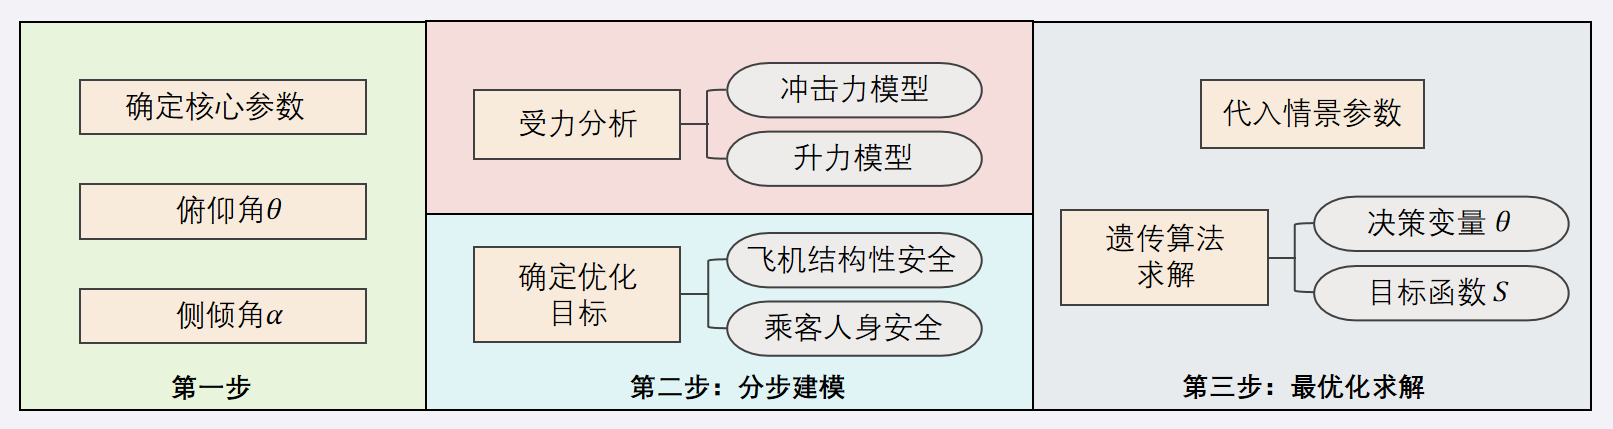
\includegraphics[width=1.0\textwidth]{fig_problem1.png}
    \caption{问题一思路导图}
    \label{fig_problem1}
\end{figure}


问题一可以视为优化问题。首先，利用各种数学指标定量地刻画出飞机迫降的安全系数，其次结合实际添加变量约束，最后可利用遗传算法对安全系数求最大值，以此进一步确定在飞机迫降过程中确立的俯仰角、侧倾角等参数。

\subsection{模型建立}
\subsubsection{核心参数确定}

通过查阅文献法，优先确定客机水面迫降时的主要风险来源以及不同的做法带来的可能后果，进而确定客机迫降时的大体姿态。

\begin{enumerate}

\item \textbf{机身结构损坏风险:} 飞机接触水面瞬间会受到巨大冲击力，若\textbf{姿态不当（如机头直接撞击、侧倾角度过大）}，可能导致机身断裂、机翼脱落等结构性损坏。例如，水平速度过大或垂直速度过快时，水的冲击力会远超机身结构承受极限，引发解体风险。

\item \textbf{乘客冲击伤害:}   
   迫降瞬间的过载 (尤其是垂直方向)可能对乘客造成颈椎、骨骼等损伤。若飞机姿态导致局部冲击力集中，乘客的\textbf{瞬时加速度}可能超过人体耐受极限 (通常认为安全阈值约5g)，导致伤亡。

\item \textbf{飞机沉没与逃生阻碍:}   
   即使迫降时结构未严重损坏，飞机仍可能因进水逐渐沉没。若舱门、紧急出口因变形无法打开，或逃生滑梯/救生筏没有成功释放，会严重阻碍乘客撤离，增加溺水风险。

\item \textbf{风浪条件下的额外风险:}  
波浪冲击可能导致飞机颠簸、侧翻，尤其是横浪 (机身与波浪传播方向垂直)时，\textbf{侧向力易使飞机失去平衡。} 风浪会加剧机身与水面的非均匀接触，导致局部受力过大，同时增加飞机姿态控制难度，可能引发二次撞击。

\end{enumerate}

综上所述，需要对飞机迫降时的姿态进行调整。根据查阅内容，可以提炼如下基本要点:

\begin{itemize}
    
    \item 需控制\textbf{俯仰角 (机头微抬)和侧倾角 (机翼水平)}。使机身后部先接触水面，分散冲击力，避免机头直接撞击导致的结构损坏；需要保持两侧机翼水平，防止因一侧机翼率先入水导致飞机翻转。
    
    \item 在有风浪的情况下，还需结合航向调整姿态。优先\textbf{选择顺浪航向 (机身与波浪传播方向一致)}，利用波浪速度降低相对冲击速度；特别地，考虑到波峰的存在，俯仰角可略大于平静水面以抵消波峰的额外冲击。

    \item 控制速度与加速度。需尽可能降低垂直速度 (减少下落冲击)和水平速度 (减少滑行时的摩擦与撞击力)，但需保持足够升力使飞机姿态稳定，避免失速。尽量使整个过程加速度在人体可承受范围内。

\end{itemize}

问题一水面平静，将水面视为\textbf{理想刚性平面}，冲击力仅与接触面积、速度和姿态相关。
飞机需要尾部优先接触水面，将其视为\textbf{刚体}。含机身 (长$L$、宽$W$、高$H$)、机翼 (展长$B$、面积$S$)。
飞机与货物总质量为$m$。

为了评价迫降姿态的安全性，引入俯仰角和侧倾角两个核心参数:

\begin{itemize}

    \item \textbf{俯仰角$\theta$}: 机身纵轴与水面的夹角，$\theta>0$为机头抬起，$\theta<0$为机头俯冲。

    \item \textbf{侧倾角$\alpha$}: 机翼平面与水面的夹角，依据资料内容, 机翼应当水平，即$\alpha=0$。
    
\end{itemize}
    

\subsubsection{分步建模}


 \paragraph{1. 冲击力模型}
    飞机接触水面时，水的阻力可简化为\textbf{动量定理}:
    
    \begin{equation}
     f = k \cdot \frac{\Delta p}{\Delta t} 
    \label{FormulaOfF}
    \end{equation}

    其中 $\Delta p$ 是流体动量变化，$\Delta t$ 是作用时间，$k$为经验系数，依据流体撞击试验确定，常见的取值范围为$0.5 \sim 1.0$。

    
\begin{figure}[H]
    \centering
    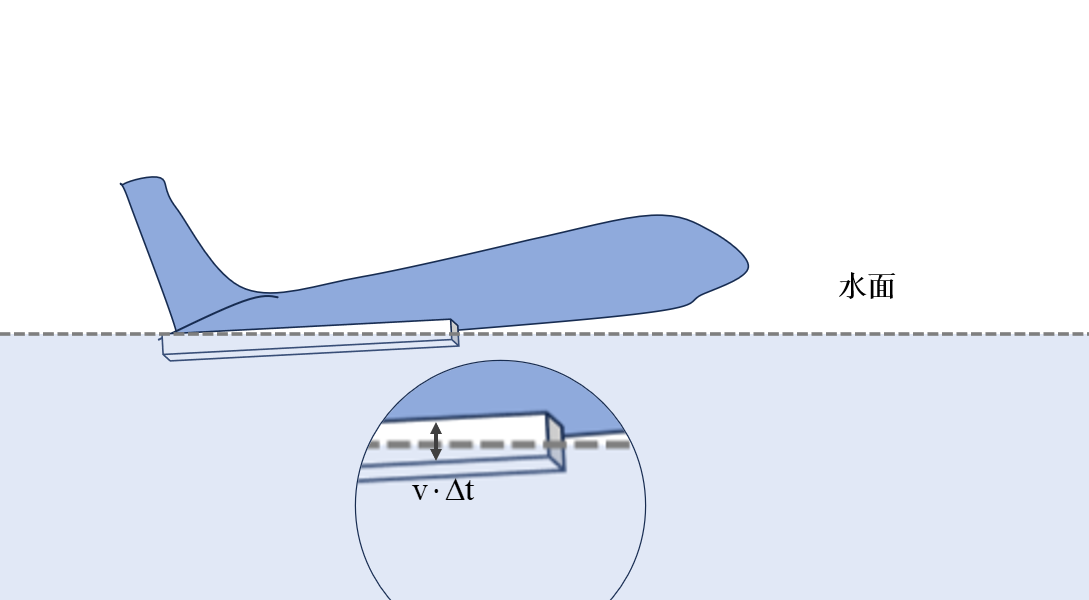
\includegraphics[width=0.8\textwidth]{fig_theDifferentialA.png}
    \caption{冲击力模型的微分形式}
    \label{fig:aircraft_dim}
\end{figure}

    假设飞机接触水面时，\textbf{瞬时推开的水体积为 $V$}，这些水的速度从 $0$ 被加速到与飞机接近的速度 $v$。   
    推开的水体积 $V$与 \textbf{瞬时接触面积 $A$} 和 \textbf{作用距离} 相关。   
    飞机在极短时间 $\Delta t$ 内，以速度 $v$ 挤压水, 推开的水可近似为"柱体"，柱体高度为 $v \cdot \Delta t$. 
    因此，体积 $V \approx A \cdot (v \cdot \Delta t)$。 
    
    则动量变化: 
    
    \begin{equation}
    \Delta p = m \cdot v = \rho \cdot V \cdot v \approx 
    \rho \cdot A \cdot (v \cdot \Delta t) \cdot v 
    \label{FormulaOfDeltaP}
    \end{equation}

    在式\eqref{FormulaOfDeltaP}中, $A$为瞬时接触面积, 表达式为

    \begin{equation}
        A = W \cdot l_t = W \cdot \frac {\int_{0}^{t} v_v dt}{\sin\theta}
        \label{FormulaOfA}
    \end{equation}


\begin{figure}[H]
    \centering
    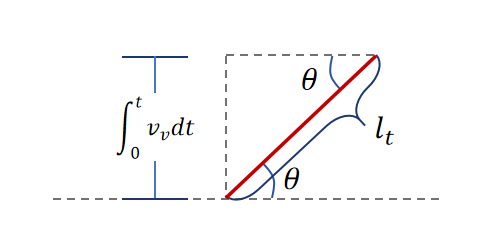
\includegraphics[width=0.7\textwidth]{fig_l_t.png}
    \caption{$l_t$的几何关系}
    \label{fig:aircraft_dim}
\end{figure}


    $A$与$\theta$、$\alpha$相关，由已知条件分析得$\alpha = 0$, 对$A$的求解无影响. 在$\theta=0$时$A$为机身底部投影面积.  
    其中，仅机身后部接触水面时，$l_t = \frac{\int_{0}^{t} v_v dt}{\sin\theta}$
    为机身与水面的实际接触段长度（非机身全长）. 
    $\int_{0}^{t} v_v dt$为从飞机接触水面开始到t时刻的垂直位移 (机身下沉深度). 
    

    由式\eqref{FormulaOfF}\eqref{FormulaOfDeltaP}\eqref{FormulaOfA}得
    \begin{equation}
    f = k \cdot \rho \cdot W \cdot \frac {\int_{0}^{t} v_v dt}{\sin\theta} \cdot v^2 
    \label{TheFnalF}
    \end{equation}

    其中：
\begin{itemize}

\item $\rho$为水的密度 ($1025\ \text{kg/m}^3$). 

\item $W$为机体宽度. 

\item $v$为接触点相对水面的合速度($v=\sqrt{v_h^2 + v_v^2}$，迫降速度分解为：水平速度$v_h$（沿机身纵轴）、垂直速度$v_v$ (竖直向下)。
). 

\end{itemize}


\paragraph{2. 受力分析}

除了水流的冲击力外，飞机自身受到升力和重力作用。在最优迫降姿态下，侧倾角$\alpha = 0 $，因此升力的方向垂直水面向上，其计算公式为
\begin{equation}
    L = \frac{1}{2} \eta \cdot \rho_{\text{air}} \cdot v_h^2 \cdot S \cdot C_L
    \label{FormulaOfL}
\end{equation}

其中:  
\begin{itemize}
    \item $\eta$为升力衰减系数, 与接触面积$A$以及机翼面积$S$相关, 依据具体实验测定, 描述了在飞机触水时升力的损耗情况.
    \item $\rho_{\text{air}}$为空气密度 (约 $1.225 \, \text{kg/m}^3$).   
    \item $v_h$为飞机水平速度.   
    \item $S$为机翼面积.   
    \item $C_L$为升力系数.   
\end{itemize}

\begin{figure}[htbp]
    \centering
    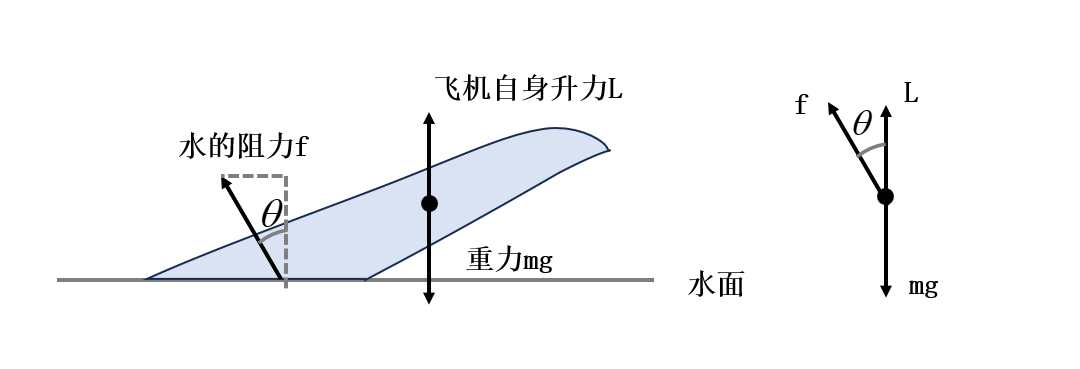
\includegraphics[width=0.8\textwidth]{fig_force_analysis.png}
    \caption{客机水面迫降受力分析示意图 (升力$L$、重力$mg$、水阻力$f$)}
    \label{fig:force_analysis}
\end{figure}

对飞机的受力正交分解。竖直方向上受力为$F_v$，水平方向上受力为$F_h$，其表达形式如下. 
\begin{equation}
    F_v = mg - L - f \cdot \cos\theta
    \label{F_v}
\end{equation}
\begin{equation}
    F_h = f \cdot \sin\theta
    \label{F_h}
\end{equation}


\paragraph{3. 安全性指标} 依据4.2.1的风险来源，确定下述指标. 

\begin{itemize}

\item \textbf{结构损伤风险}: 机身最大弯矩$M_{\text{max}}\leq M_{\text{lim}}$ 

\end{itemize}
   \begin{equation}
    M_{\text{max}} = f \cdot d
    \label{FormulaOfM_max}
    \end{equation}

    当实际弯矩$M_{\text{max}} \leq M_{\text{lim}}$时，机身可避免结构性断裂或解体。
    其中，$d$为冲击力作用点到机身重心的水平距离，$M_{\text{lim}}$是客机机身结构在迫降冲击下所能承受的最大弯矩临界值。

   将客机机身简化为\textbf{变截面空心圆柱壳结构} (忽略局部凸起，如舷窗、舱门)，材料的屈服强度为$\sigma_s$，弹性模量为$E$。设机身某截面的外径为$D$、内径为$d$ (壁厚$t=\frac{D-d}{2}$)。
   
   截面惯性矩为
    
   \begin{equation}
   I = \frac{\pi}{64}(D^4 - d^4)
   \label{FormulaOfI}
   \end{equation}

   截面抵抗矩为
   
   \begin{equation}
   W = \frac{2I}{D}
    \label{FormulaOfW}
    \end{equation}
   
  根据材料力学中弯曲强度条件，极限弯矩公式为
   \begin{equation}
    M_{\text{lim}} = \sigma_s \cdot W_{\text{resist}}
    \label{FormulaOfM_lim}
    \end{equation}

  由式\eqref{FormulaOfI}\eqref{FormulaOfW}\eqref{FormulaOfM_lim}得

  \begin{equation}
  M_{\text{lim}} = \sigma_s \cdot \frac{\pi}{32} \cdot \frac{D^4 - d^4}{D}
    \label{formulaOfM_lim}
  \end{equation}
  
  对于机身不同位置, 因截面尺寸不同, $M_{\text{lim}}$需分段计算, 取最小值作为整体结构的临界值. 


\begin{itemize}

\item \textbf{乘客过载}: 竖直方向加速度$a_v$与水平方向加速度$a_h$受限,  
需满足$a_v < 3g$, $a_h < 5g$ (普通人耐受极限). 

\end{itemize}

\begin{equation}
a_v = \frac{F_v}{m} 
\label{a_v}
\end{equation}
\begin{equation}
a_h = \frac{F_h}{m} 
\label{a_h}
\end{equation}


由式\eqref{TheFnalF}\eqref{FormulaOfL}\eqref{F_v}\eqref{a_v}可得 

\begin{equation}
\frac{dv_v}{dt} = a_v = \frac{mg - L - f\cos\theta}{m} = 
g - \frac{\eta \rho_{\text{air}} S C_L \cdot v_h^2}{2m} - 
k \cdot \frac{\rho \cos\theta \cdot A \cdot v^2}{m}
\label{frac1}
\end{equation}

由式\eqref{TheFnalF}\eqref{F_h}\eqref{a_h} 可得

\begin{equation}
\frac{dv_h}{dt} = a_h = \frac{fsin\theta}{m} =
 k \cdot \frac{\rho \sin\theta \cdot A \cdot v^2}{m}
\label{frac2}
\end{equation}

式\eqref{frac1}\eqref{frac2}满足

\begin{equation}
\left(\frac{dv}{dt}\right)^2=\left(\frac{dv_v}{dt}\right)^2 + \left(\frac{dv_h}{dt}\right)^2
\label{dv_dt} 
\end{equation}

式\eqref{dv_dt}建立起了水平方向与竖直方向的联系, 式中的相关变量均与速度$v$建立了联系, 
并且在具体情境下可将初速度$v_{v0}$与$v_{h0}$与俯仰角$\theta$建立联系. 从而
将各个变量和俯仰角$\theta$关联. 

\subsection{情景求解}
\subsubsection{代入初始参数}
以2009 年1 月15 日下午, US Airways 所属第1549 航班 (空中客车A320 客机)为例，其参数如下。

\begin{table}[H]
\centering
\caption{A320 客机主要参数}
\label{tab:a320_params}
\begin{tabular}{|m{2cm}|m{4cm}|m{4cm}|}

\hline
\textbf{参数类别} & \textbf{具体参数} & \textbf{数值/说明} \\ 
\hline
\multirow{8}{*}{\textbf{尺寸参数}} 
& 机身长度 & 37.57 米 \\ \cline{2-3}
& 机身宽度 & 3.95 米 \\ \cline{2-3}
& 翼展（几何尺寸） &  35.8 米 \\ \cline{2-3}
& 机翼面积 & 122.4 平方米 \\ \cline{2-3}
& 客舱长度 & 27.74 米 \\ \cline{2-3}
& 客舱宽度 & 3.7 米 \\  \cline{2-3} 
& 机身高度 & 11.76米 \\ \cline{2-3}
& 机身厚度 & 0.05米 \\ 
\hline
\multirow{3}{*}{\textbf{材料参数}}
& 主要材料 &  7075 - T6 铝合金 \\ \cline{2-3}
& 屈服强度 &  460MPa \\ \cline{2-3}
& 弹性模量  &  70GPa \\ 
\hline
\multirow{3}{*}{飞行参数}
& 最大升力系数 & 1.662 \\ \cline{2-3}
& 升力衰减系数  & max(0.2, 1 - A / S) \\ \cline{2-3}
& 冲击模型经验系数  & 0.8 \\
\hline
\end{tabular}
\end{table}


\begin{figure}[H]
    \centering
    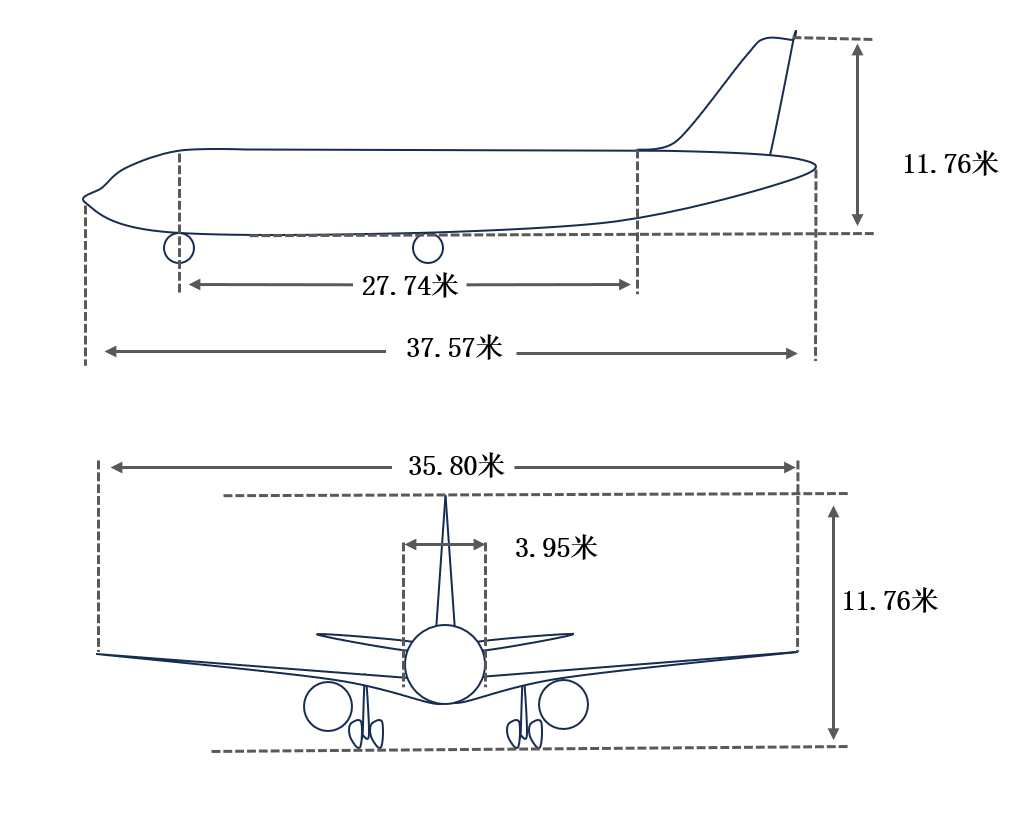
\includegraphics[width=0.8\textwidth]{fig_aircraft_dimension.png}
    \caption{A320客机尺寸参数 (侧视图与正视图)}
    \label{fig:aircraft_dim}
\end{figure}

由表\ref{tab:a320_params}知，机身长度$L = 37.57m$，机身宽度$W = 3.95m$，壁厚$0.05m$
那么机身弯矩由式\eqref{formulaOfM_lim}得
\begin{equation}
    M_{\text{lim}} = 1.726 \times 10^7 \, \text{N·m}
    \label{specfica_M_lim}
\end{equation}

初始状态下, 冲击力作用点 (即机身尾部)到机身重心的水平距离
\begin{equation}
    d \approx \frac{L}{3} = 12.523 m 
    \label{specfica_d}
\end{equation}

机翼面积$S=122.4 m^2$，飞机总质量$ m = 68700 kg $，飞机以约 130 节速度迫降, 约66.872 $m/s$, 在最优降落姿态下侧倾角$\alpha = 0 $, 那么
\begin{equation}
    v_{v0} = v_0 \cdot \cos\theta = 66.872 \cdot \cos\theta
    \label{specfica_v}
\end{equation}
\begin{equation}
     v_{h0} = v_0 \cdot \sin\theta = 66.872 \cdot \sin\theta
    \label{specfica_h}
\end{equation}


\subsubsection{遗传算法最优化结果}


通过数值模拟不同$\theta$和$\alpha$的$M_{\text{max}}$和$a_v$，得出最佳姿态。

\textbf{Step1 初始化个体与种群}

每个个体代表一个候选俯仰角 (单位：°), 是遗传算法搜索空间中的一个解. 

初始化范围可通过\textbf{lb = 0和ub = 15限定个体的取值范围为 0°~15°}, 
即所有初始个体的俯仰角均在该区间内生成，确保符合实际中飞机水上迫降的俯仰角合理范围.  
由 MATLAB 的\textbf{ga函数}默认采用\textbf{随机均匀采样方式}生成初始种群, 即在 0°~15° 的范围内随机均匀. 

\textbf{Step2 设计适应度函数}

国际民航组织 (ICAO)明确将人员安全置于首位, 遵循''安全优先、兼顾结构''准则, 综合''飞机结构性损伤''与''人员安全''两项指标, 
定义安全系数
\begin{equation}
S = \omega_1 \cdot \left(1 - \frac{M_{\text{max}}}{M_{\text{lim}}}\right) + 
\omega_2 \cdot \left(1 - \frac{a_v}{3g}\right) + 
\omega_3 \cdot \left(1 - \frac{a_h}{5g}\right)
\label{FormulaOfS}
\end{equation}

其中$\omega_1$、$\omega_2$、$\omega_3$为权重，根据结构安全与乘客安全的优先级设定
, $\omega_1=0.3$, $\omega_2=0.4$, $\omega_3=0.3$.

以安全系数$S$的负值为优化目标. 

\textbf{Step3 进化迭代}

利用由 MATLAB 内置的ga函数自动实现采用\textbf{均匀变异}, 即对种群中的个体
 (俯仰角) 以一定概率在其取值范围 (0°~15°) 内进行随机扰动, 生成新的个体. 

\textbf{Step4 终止迭代}

\begin{itemize}
\item 最大迭代次数: 当算法迭代达到 100 代时, 无论是否收敛, 都会终止迭代. 

\item 函数容差: 当相邻两代的最优目标函数值差异小于$10^{-6}$时, 算法判定为收敛, 提前终止迭代, 避免无效计算. 
\end{itemize}
符合以上条件其一即终止迭代.


通过数值模拟不同俯仰角下的安全系数, 得到安全系数最优时,
各参数如图\ref{fig:debug_info}所示. 
安全系数随俯仰角变化的曲线如图\ref{fig:safety_curve}所示. 


\begin{figure}[H]
    \centering
    
\includegraphics[width=0.9\textwidth]{fig_debug_info.png}
    \caption{A320迫降仿真调试信息 ($\theta = 7.30^\circ$时参数)}
    \label{fig:debug_info}
\end{figure}


\begin{figure}[H]
    \centering
    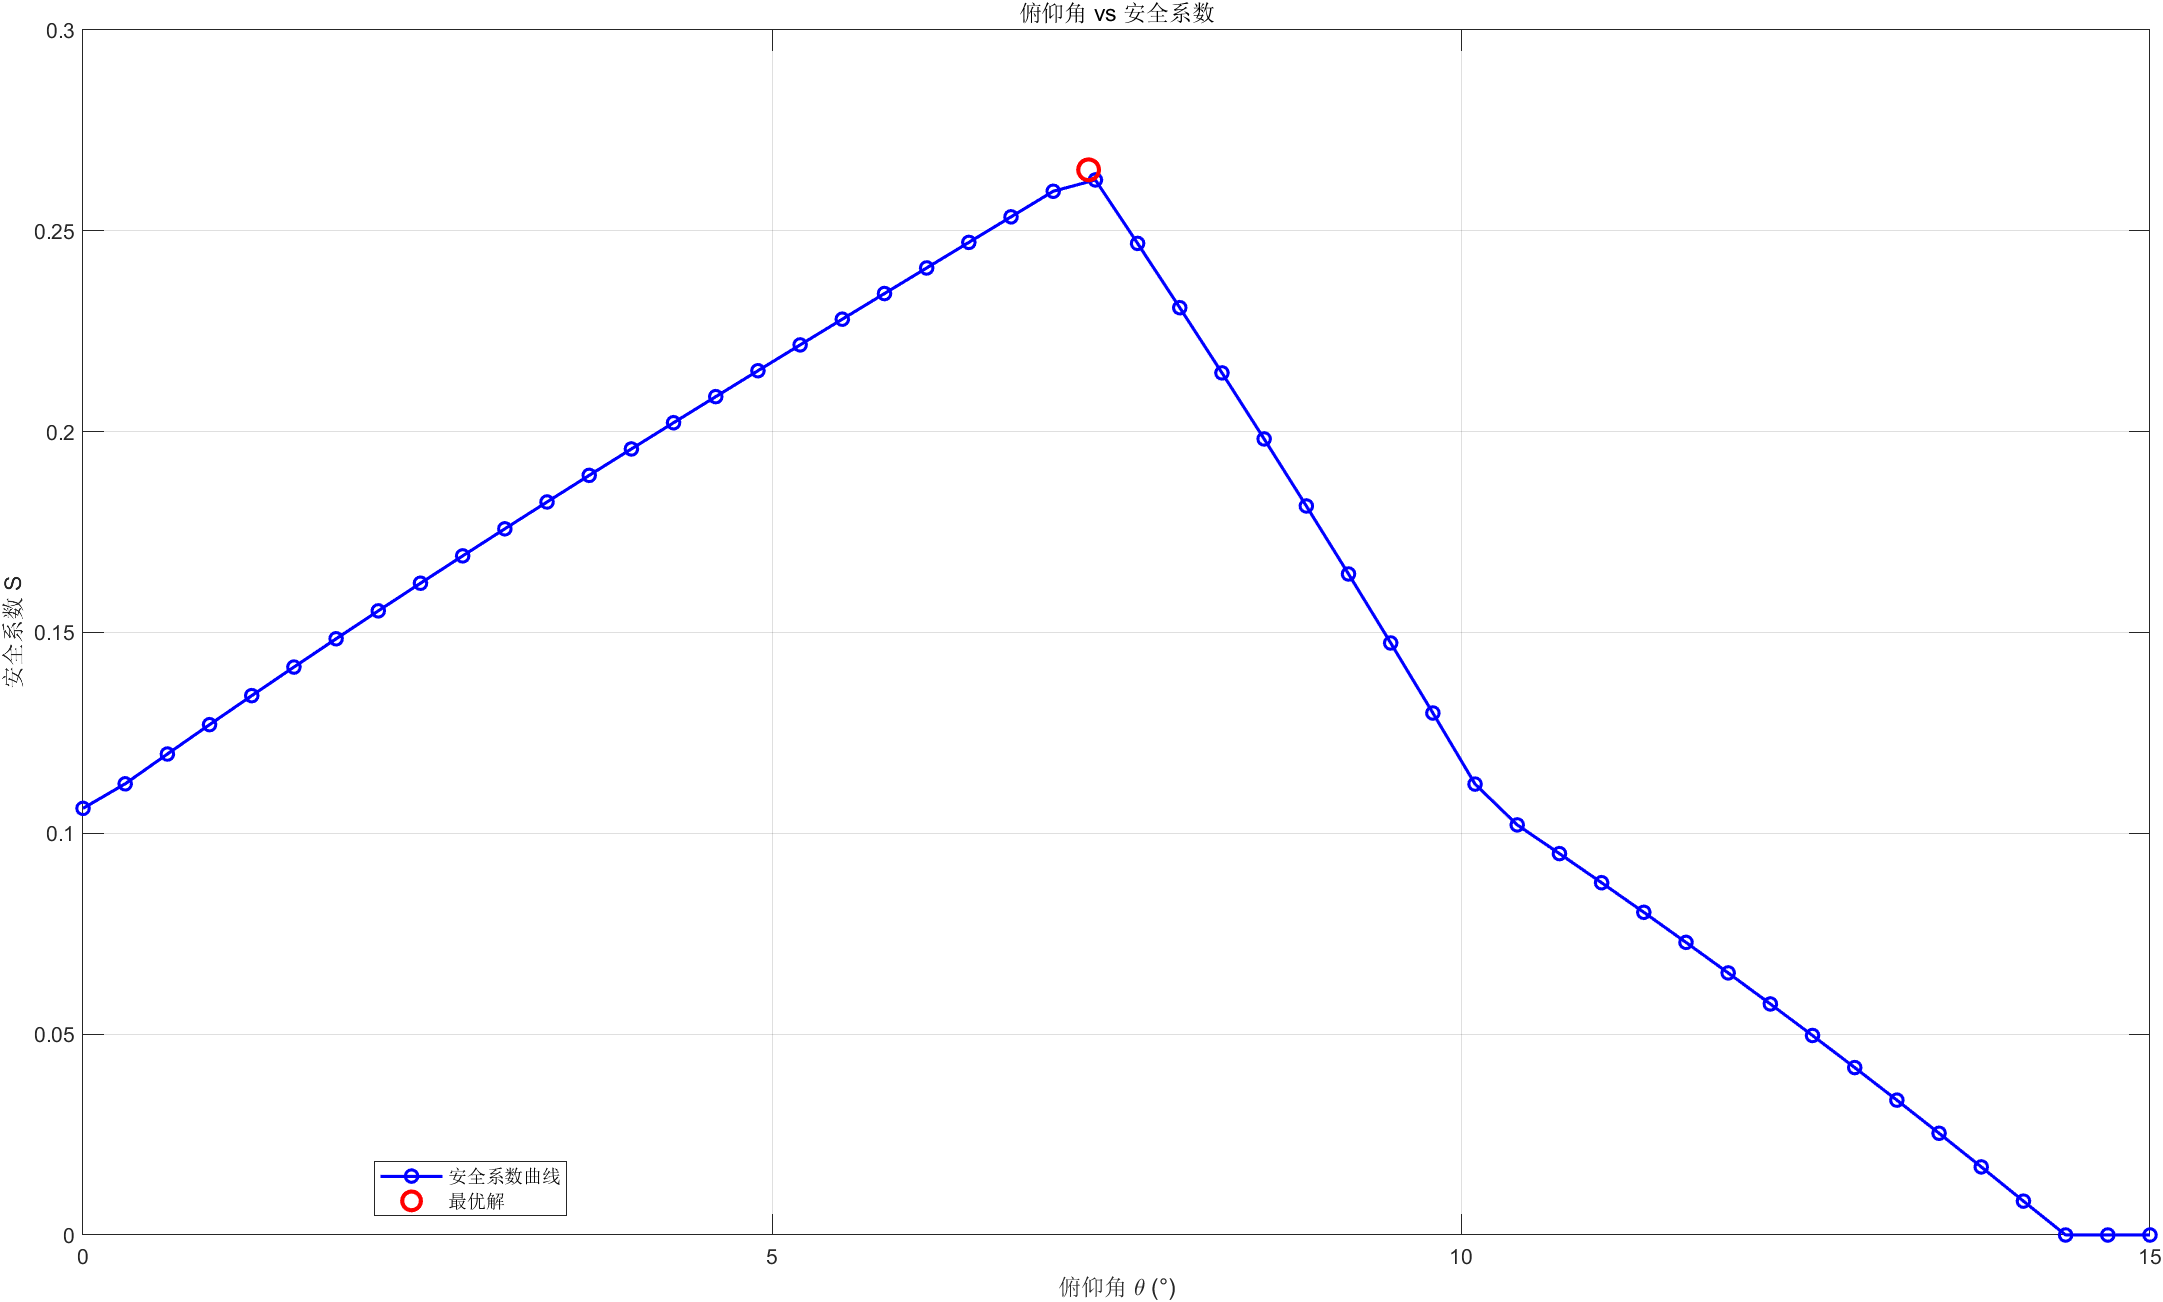
\includegraphics[width=0.8\textwidth]{fig_safety_coefficient.png}
    \caption{俯仰角$\theta$与安全系数$S$关系曲线（最优解标记）}
    \label{fig:safety_curve}
\end{figure}

由图\ref{fig:safety_curve}可知, 安全系数$S$随俯仰角$\theta$先增后减, 在$\theta \approx 7.3^\circ$时达到最大值$S=0.265$, 此时机身结构受力和乘客过载均处于较优状态, 是平静水面下的最优迫降姿态. 


\section{问题二模型建立与求解}

\subsection{问题二分析}


\begin{figure}[H]
    \centering
    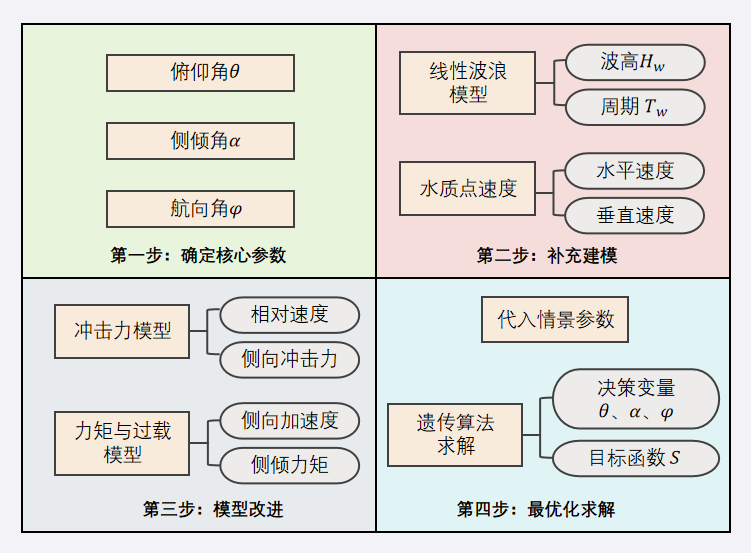
\includegraphics[width=0.8\textwidth]{fig_problem2.png}
    \caption{问题二思路导图}
    \label{fig_problem2}
\end{figure}


问题二在问题一的基础上增加了风浪条件, 并要求给出具体的航向. 因此需要引入航向角, 并对
波浪函数进行表示. 风浪存在会改变冲击力模型、瞬时接触面积等相关参数, 并带来侧向力等问题. 


\begin{table}[H]
\centering
\caption{ 问题二物理量符号及意义}
\begin{tabular}{|c|c|}
\hline
\textbf{符号} & \textbf{物理意义} \\
\hline
\(\theta\) & 俯仰角（机身纵轴与水面夹角，\(\theta>0\)为机头抬起） \\
\hline
\(\alpha\) & 侧倾角（机翼平面与水面夹角，\(\alpha=0\)为机翼水平） \\
\hline
\(\phi\) & 航向角（机身纵轴与波浪传播方向夹角，\(\phi=0^\circ\)为顺浪） \\
\hline
\(v_h, v_v, v_s\) & 飞机水平、垂直、侧向速度 \\
\hline
\(v_h', v_v', v_s'\) & 相对水面的水平、垂直、侧向速度 \\
\hline
\(f_h, f_v, f_s\) & 水平、垂直、侧向冲击力 \\
\hline
\(M_{\text{max}}, M_s\) & 机身最大弯矩、侧倾力矩 \\
\hline
\(a_v, a_h, a_s\) & 竖直、水平、侧向加速度 \\
\hline
\(H_w, T_w\) & 波高、波浪周期 \\
\hline
\end{tabular}
\end{table}

\subsection{模型引入}

\subsubsection{线性波浪模型}



\begin{comment}
小振幅假设：波浪的振幅远小于波长，且远小于水深，因此可以忽略运动方程中的高阶非线性项。

势流假设：假设流体是无粘性、不可压缩的，波浪运动可以用速度势函数描述，从而简化控制方程。
\end{comment}


波浪运动本质上是流体在重力、表面张力等作用下的复杂运动，
其控制方程是非线性的，直接求解难度极大。考虑到问题二是在海洋表面迫降,
水深\(h \gg \lambda\), 符合线性波浪模型的深水特点, 此时波浪运动主要集中
在水面附近，底部影响可忽略。

故采用线性波浪模型简化问题, 查阅资料得, 对于一个
波高$H_w$、周期$T_w$、传播方向$\psi$, 波速$c$. 线性波浪模型的色散关系满足
\begin{equation}
    \omega^2 = gk \tanh(kh)
    \label{seSanGuanXi}
\end{equation}

其中, $k=\frac{2\pi}{\lambda}$为波数, $\omega$为圆频率, $h$为水深, $tanh$是双曲正切函数.
当水深 \( h \) 足够大时, \( kh \gg 1 \), 则$\tanh(kh) \approx 1$, 深水条件下的色散关系简化为：
\begin{equation}
    \omega^2 \approx gk
    \label{simpleSeSanGuanXi}
\end{equation}
将 \( \omega = \frac{2\pi}{T_w} \) 和 \( k = \frac{2\pi}{\lambda} \) 代入式\eqref{simpleSeSanGuanXi}得
\begin{equation}
    \left( \frac{2\pi}{T_w} \right)^2 = g \cdot \frac{2\pi}{\lambda}
    \label{simpleSeSanGuanXi1}
\end{equation}
    化简式\eqref{simpleSeSanGuanXi1}得
\begin{equation}
     \lambda = \frac{g T_w^2}{2\pi} 
    \label{FormulaOfLambda}
\end{equation}
    那么对给定周期的波浪, 可大致推算出其波长. 

\begin{table}[h]
    \centering
    \caption{波浪参数表} 
    \begin{tabular}{|c|c|c|c|c|}
        \hline
        强度 & $H_w (m)$ & $T_w (s)$ & $\lambda (m)$ & $C_w (m/s)$ \\
        \hline
        微弱 & 1 & 5 & 39.01 & 7.8  \\
        \hline
        普通 & 2 & 10 & 156.05 & 15.6 \\
        \hline
        强风浪 & 10 & 20 & 624.20 & 31.2  \\
        \hline
    \end{tabular}
    \label{tab:wave_params} 
\end{table}



\subsubsection{水质点模型}

在深水线性波浪中, 水质点做周期性圆周运动, 其运动轨迹可表示为: 在波峰处水质点向上运动, 波谷处向下运动,
水平方向则随波浪传播方向往复运动. 水质点速度可分解为水平速度$u_w$与垂直速度$w_w$

\begin{figure}[H]
    \centering
    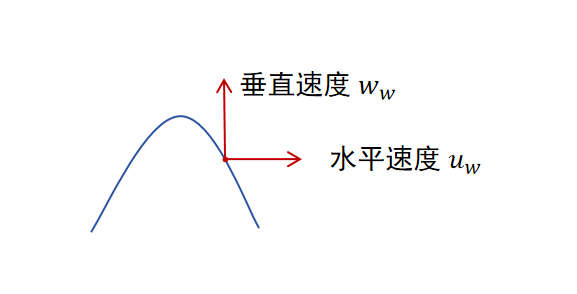
\includegraphics[width=0.6\textwidth]{fig_speed_analysis.png}
    \caption{水质点速度分解}
    \label{fig_speed}
\end{figure}
\begin{equation}
    u_w=\frac{\pi H_w}{T_w} \cdot e^{kz}
    \label{u_w}
\end{equation}
\begin{equation}
    w_w=\frac {\pi H_w}{T_w} \cdot e^{kz}
     \label{w_w}
\end{equation}

\subsection{模型改进}
\subsubsection{冲击力模型}

\begin{figure}[H]
    \centering
    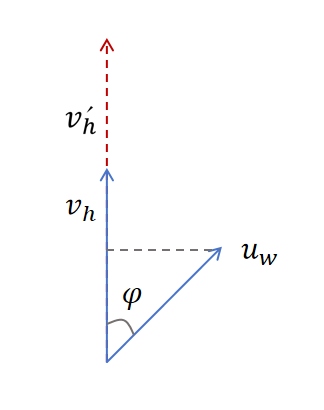
\includegraphics[width=0.2\textwidth]{fig_relativespeed.png}
    \caption{水平相对速度合成示意图}
    \label{fig:relativespeed}
\end{figure}


引入风浪后, 水流自身具有速度, 依据冲量的物理意义, 需要计算相对速度. 
如图\ref{fig:relativespeed} 所示, 则各个方向上的相对速度如下

\begin{equation}
    \begin{cases}
    v_h' = v_h - u_w \cos\phi  \\
    v_v' = v_v - w_w \\
    v_s' = v_s + u_w \sin\phi 
    \end{cases}
    \label{gatherOfRelativeSpeed}
\end{equation}

基于式\eqref{FormulaOfF}\eqref{FormulaOfDeltaP}, 水平、垂直、侧向的冲击力依次为

\begin{equation}
    \begin{cases}
        f_h = k \rho A_h (v_h')^2 \\
        f_v = k \rho A_v (v_v')^2 \\
        f_s = k_s \rho A_s (v_s')^2
    \end{cases}
    \label{gatherOff}
\end{equation}
其中, $A_h$为纵向接触面积, $A_v$为垂直投影面积, $A_s$为侧向接触面积, $k_s$为侧向系数.

\subsubsection{力矩与过载计算}

力矩要求细分为机身弯矩和侧倾力矩.
\begin{equation}
    \begin{cases}
        M_{\text{max}} = f_h \cdot d_h  \\
        M_s = f_s \cdot d_s
    \end{cases}
    \label{gatherOfM}
\end{equation}
其中, $d_h$为冲击力到重心距离, $d_s$为侧向力到重心距离, 

加速度细分为水平, 垂直, 侧向三个方向. 
\begin{equation}
    \begin{cases}
    a_v = \dfrac{mg - L - f_v \cos\theta}{m} \\
    a_h = \dfrac{f_h \sin\theta}{m} \\
    a_s = \dfrac{f_s}{m}
    \end{cases}
    \label{gatherOfa}
\end{equation}
式\eqref{gatherOfRelativeSpeed}\eqref{gatherOff}
\eqref{gatherOfM}\eqref{gatherOfa}和水质点模型建立关联, 
从而引入海浪因素. 

\subsection{情景求解}


\subsubsection{安全系数定义}
\[
S = \omega_1\left(1 - \frac{M_{\text{max}}}{M_{\lim}}\right) + 
\omega_2\left(1 - \frac{a_v}{3g}\right) + \omega_3\left(1 - \frac{a_h}{5g}\right) 
+ \omega_4\left(1 - \frac{M_s}{M_{s\lim}}\right) + \omega_5\left(1 - 
\frac{a_s}{6g}\right)
\]
权重取值：$\omega_1=0.2, \omega_2=0.2, \omega_3=0.2, \omega_4=0.2, \omega_5=0.2$。

\subsubsection{约束条件}

姿态范围：$\theta \in [5^\circ, 15^\circ], \alpha \in [-3^\circ, 3^\circ], \phi \in [0^\circ, 30^\circ]$

速度约束：$v_h \leq 70\,\text{m/s}, v_v \leq 3\,\text{m/s}$

\subsubsection{优化目标}
通过遗传算法最大化安全系数$S$，求解最优参数$(\theta^*, \alpha^*, \phi^*)$。

\subsection{结论}





%参考文献
\begin{thebibliography}{9}%宽度9
   
\end{thebibliography}

\newpage
%附录
\begin{appendices}

\section{模板所用的宏包}
\begin{table}[htbp]
    \centering
    \caption{宏包罗列}
    \begin{tabular}{ccccc}
        \toprule
        \multicolumn{5}{c}{模板中已经加载的宏包} \\
        \midrule
        amsbsy & amsfonts & {amsgen} & {amsmath} & {amsopn} \\
        amssymb & amstext & {appendix} & {array} & {atbegshi} \\
        atveryend & auxhook & {bigdelim} & {bigintcalc} & {bigstrut} \\
        bitset & bm    & {booktabs} & {calc} & {caption} \\
        caption3 & CJKfntef & {cprotect} & {ctex} & {ctexhook} \\
        ctexpatch & enumitem & {etexcmds} & {etoolbox} & {everysel} \\
        expl3 & fix-cm & {fontenc} & {fontspec} & {fontspec-xetex} \\
        geometry & gettitlestring & {graphics} & {graphicx} & {hobsub} \\
        hobsub-generic & hobsub-hyperref & {hopatch} & {hxetex} & {hycolor} \\
        hyperref & ifluatex & {ifpdf} & {ifthen} & {ifvtex} \\
        ifxetex & indentfirst & {infwarerr} & {intcalc} & {keyval} \\
        kvdefinekeys & kvoptions & {kvsetkeys} & {l3keys2e} & {letltxmacro} \\
        listings & longtable & {lstmisc} & {ltcaption} & {ltxcmds} \\
        multirow & nameref & {pdfescape} & {pdftexcmds} & {refcount} \\
        rerunfilecheck & stringenc & {suffix} & {titletoc} & {tocloft} \\
        trig  & ulem  & {uniquecounter} & {url} & {xcolor} \\
        xcolor-patch & xeCJK & {xeCJKfntef} & {xeCJK-listings} & {xparse} \\
        xtemplate & zhnumber &       &       &  \\
        \bottomrule
    \end{tabular}%
    \label{tab:addlabel}%
\end{table}%

以上宏包都已经加载过了，不要重复加载它们。

\section{问题一：遗传算法}

\begin{lstlisting}[language=matlab]
	
%% 飞机水上迫降最优俯仰角求解
clear; close all; 

%% 飞机及环境参数
L = 37.57;          % 机身长度 (m)
W = 3.95;           % 机身宽度 (m)
S_wing = 122.4;     % 机翼面积 (m^2)
m = 68700;          % 质量 (kg)
rho_air = 1.225;    % 空气密度 (kg/m^3)
rho_water = 1025;   % 水密度 (kg/m^3)
CL = 1.662;         % 升力系数
v0 = 66.872;            % 初始速度 (m/s) 
g = 9.81;           % 重力加速度 (m/s^2)
k = 0.8;            % 冲击经验系数

% 材料截面参数
sigma_s = 460e6;    % 屈服强度 (Pa)
D_outer = 3.95;     % 外径 (m)
t_wall = 0.05;      % 壁厚 (m)
d_inner = D_outer - 2*t_wall;
I = (pi/64) * (D_outer^4 - d_inner^4);
W_resist = 2 * I / D_outer;
Mlim = sigma_s * W_resist;  % 极限弯矩 (N·m)

% 权重分配
w1 = 0.3;   % 弯矩权重
w2 = 0.4;   % 竖直加速度权重
w3 = 0.3;   % 水平加速度权重

% 安全系数函数句柄
safety_fun = @(theta_deg) calcSafety(theta_deg, L, W, S_wing, m, rho_air, rho_water, ...
    CL, v0, g, k, Mlim, w1, w2, w3, false);

%% 遗传算法设置
lb = 0; ub = 15;    % 俯仰角搜索范围 (deg)
opts = optimoptions('ga', ...
    'PopulationSize', 50, ...
    'MaxGenerations', 100, ...
    'Display', 'iter', ...
    'FunctionTolerance', 1e-6);

% 目标函数（
obj_fun = @(theta) -safety_fun(theta);

[theta_opt, S_opt_neg] = ga(obj_fun, 1, [], [], [], [], lb, ub, [], opts);
S_opt = -S_opt_neg;

% 输出最优解并打印调试信息
[~, Mmax_opt, av_opt, ah_opt] = calcSafety(theta_opt, L, W, S_wing, m, rho_air, rho_water, ...
    CL, v0, g, k, Mlim, w1, w2, w3, true);

fprintf('\n=== 最优结果 ===\n');
fprintf('最优俯仰角 θ = %.4f°\n', theta_opt);
fprintf('最大弯矩 Mmax = %.4f MN·m (极限 %.4f MN·m)\n', Mmax_opt/1e6, Mlim/1e6);
fprintf('竖直加速度 av = %.4f g (向下为正)\n', av_opt/g);
fprintf('水平加速度 ah = %.4f g(向前为正)\n', ah_opt/g);
fprintf('安全系数 S = %.6f\n', S_opt);

%% 绘制安全系数曲线
theta_list = linspace(lb, ub, 50);
S_list = arrayfun(safety_fun, theta_list);

figure;
plot(theta_list, S_list, 'b-o', 'LineWidth', 1.5);
xlabel('俯仰角 \theta (°)');
ylabel('安全系数 S');
title('俯仰角 vs 安全系数');
grid on;
hold on;
plot(theta_opt, S_opt, 'ro', 'MarkerSize', 10, 'LineWidth', 2);
legend('安全系数曲线', '最优解', 'Location', 'best');

%% 辅助函数：计算安全系数
function [S, Mmax, av_down, ah] = calcSafety(theta_deg, L, W, S_wing, m, rho_air, rho_water, ...
    CL, v0, g, k, Mlim, w1, w2, w3, debugPrint)

    theta = deg2rad(theta_deg);
    
    % 速度分解
    vh = v0 * cos(theta);  % 水平分量
    vv = v0 * sin(theta);  % 垂直分量
    
    % 动态最小接触比例（随角度增大而减小）
    min_frac = max(0.05, 0.2 - 0.01*theta_deg);
    lt_geom = L * sin(theta);
    lt = max(lt_geom, min_frac * L);
    A_contact = W * lt;
    
    % 升力模型（考虑触水后衰减）
    eta = max(0.2, 1 - A_contact / S_wing);  % 升力衰减因子
    Lift = eta * 0.5 * rho_air * (vh^2 + vv^2) * S_wing * CL;
    
    % 冲击力模型（混合速度依赖）
    f_vertical = k * rho_water * A_contact * (vv^2 + 0.2 * vh^2);
    f_horizontal = -0.1 * f_vertical;
    
    % 加速度计算
    av_down = (m*g - Lift - f_vertical) / m;  % 向下为正
    ah = f_horizontal / m;
    
    % 最大弯矩（力臂取L/3更符合实际压力分布）
    Mmax = f_vertical * (L/3);
    
    % 安全项（限制条件更严格）
    term1 = max(0, min(1, 1 - Mmax / Mlim));              % 弯矩项
    term2 = max(0, min(1, 1 - abs(av_down) / (3 * g)));   % 竖直加速度限3g
    term3 = max(0, min(1, 1 - abs(ah) / (5 * g)));        % 水平加速度限5g
    S = w1 * term1 + w2 * term2 + w3 * term3;
    
    % 调试输出
    if debugPrint
        fprintf('\n=== 调试信息 θ = %.2f° ===\n', theta_deg);
        fprintf('速度: vh=%.2f m/s, vv=%.2f m/s\n', vh, vv);
        fprintf('接触面积: lt=%.2f m, A=%.2f m²\n', lt, A_contact);
        fprintf('升力衰减因子 eta=%.2f\n', eta);
        fprintf('修正后升力: %.2e N (%.2f倍重量)\n', Lift, Lift/(m*g));
        fprintf('修正后冲击力: f_vertical=%.2e N, f_horizontal=%.2e N\n', f_vertical, f_horizontal);
        fprintf('加速度: av=%.2f g (向下), ah=%.2f g(向前)\n', av_down/g, ah/g);
        fprintf('弯矩: Mmax=%.2e N·m (%.2f%% 极限)\n', Mmax, 100*Mmax/Mlim);
        fprintf('安全项: term1=%.3f, term2=%.3f, term3=%.3f\n', term1, term2, term3);
    end
end

 \end{lstlisting}

 \section{规划解决程序--lingo源代码}

\begin{lstlisting}[language=c]
kk=2;
[mdd,ndd]=size(dd);
while ~isempty(V)
    [tmpd,j]=min(W(i,V));tmpj=V(j);
for k=2:ndd
    [tmp1,jj]=min(dd(1,k)+W(dd(2,k),V));
    tmp2=V(jj);tt(k-1,:)=[tmp1,tmp2,jj];
end
    tmp=[tmpd,tmpj,j;tt];[tmp3,tmp4]=min(tmp(:,1));
if tmp3==tmpd, ss(1:2,kk)=[i;tmp(tmp4,2)];
else,tmp5=find(ss(:,tmp4)~=0);tmp6=length(tmp5);
if dd(2,tmp4)==ss(tmp6,tmp4)
    ss(1:tmp6+1,kk)=[ss(tmp5,tmp4);tmp(tmp4,2)];
else, ss(1:3,kk)=[i;dd(2,tmp4);tmp(tmp4,2)];
end;
end
    dd=[dd,[tmp3;tmp(tmp4,2)]];V(tmp(tmp4,3))=[];
    [mdd,ndd]=size(dd);
    kk=kk+1;
end;
S=ss;
D=dd(1,:);
 \end{lstlisting}
\end{appendices}

\end{document} 